
\documentclass{avocado}


\usepackage[ngerman]{babel}
\usepackage[german=quotes]{csquotes}
\usepackage{float}
%\usepackage{bibgerm}
\usepackage{amsmath}
\usepackage{tabularx}
\usepackage{graphicx}
\usepackage{pdflscape}
\usepackage[backend=biber, style=ieee]{biblatex}
\addbibresource{sources.bib}
%\usepackage[fixlanguage]{babelbib}
%\selectbiblanguage{german}
%\bibliographystyle{ieeetr}
%\addbibresource{sources}
\newcommand{\mail}[1]{\href{mailto:#1}{#1}}
\setlength{\parindent}{0cm}

\newcommand{\titel}{Avocado Share}
\newcommand{\shorttitel}{}
\newcommand{\doctype}{Pflichtenheft}
\newcommand{\untertitel}{Studentenplattform zum Know-How-Transfer}
\newcommand{\datum}{\today}
\newcommand{\team}{Gruppe 13}
\newcommand{\autorA}{Bergmann Sascha}
\newcommand{\autorB}{Kunz Lion}
\newcommand{\autorC}{Ngueyen Dang Thien}
\newcommand{\autorD}{Müller Cyril}
\newcommand{\autorE}{}
\newcommand{\ort}{Winterthur}
\newcommand{\dozent}{}
\newcommand{\betreuer}{}
\newcommand{\version}{1.2}

\hypersetup{
    bookmarks=false,    % show bookmarks bar?
    pdftitle={\titel - \doctype},    % title
    pdfauthor={\autorA, \autorB, \autorC, \autorD},  % author
    pdfsubject={Funktionale und nicht-funktionale Anforderungen}, % subject of the document
    pdfkeywords={\titel, \doctype, \team, Version \version, PSIT, IT15b}, % list of keywords
    colorlinks=true,        % false: boxed links; true: colored links
    linkcolor=blue!30!black,% color of internal links
    citecolor=black,        % color of links to bibliography
    filecolor=black,        % color of file links
    urlcolor=black,         % color of external links
    linktoc=page            % only page is linked
}%

%\project{Avocado Share}
\title{\title}
\author{\autorA \and \autorB \and \autorC \and \autorD \and \autorD}

\newcommand{\printrequirement}[2]{%
    \texttt{/#1/} #2% 
}

\newcommand{\requirementsection}[2]{%
    \section{\printrequirement{#1xxxx}{#2}}%
}


\newcommand{\requirementsubsection}[2]{%
    \subsection{\printrequirement{#1xx}{#2}}% 
}


\newcommand{\requirement}[2]{%
% #1: The requirement number e.g. "T0100"
% #2: The requirement title
    \subsubsection*{\printrequirement{#1}{#2}}%
    \expandafter\def\csname RequirementName#1\endcsname{#2}
    \expandafter\def\csname RequirementNumber#2\endcsname{#1}
    \label{subsub:requirement_#2}
}

% Refer to a requirement by it's title
\newcommand{\refreq}[1]{\nameref{subsub:requirement_#1}}
\newcommand{\tbf}{\emph{Noch zu definieren.}}



\usepackage[toc, xindy]{glossaries}
%\newglossary[glignoredl]{ignored}{glignored}{glignoredin}{Ignored Glossary}


\makeglossaries


\begin{document}
\newglossaryentry{Captcha}
{
	name=CAPTCHA,
	description={
		englisch für "`Completely Automated Public Turing test to tell Computers and Humans Apart"' ("`vollautomatischer öffentlicher Turing-Test zur Unterscheidung von Computern und Menschen"'), ist ein Test, welcher Benutzer lösen müssen, um zu bestätigen, dass sie keine Maschine sind
	}
}


%\newglossaryentry{ZHAW}
%{
%	name=ZHAW,
%	description={
%		Zürcher Hochschule für Angewandte Wissenschaften ist eine technische Fachhoschle in der Schweiz%
%	}
%}

\newglossaryentry{Salt}
{
	name=Salt,
	description={ist in der Informatik eine zufällig generierte Zeichenfolge, welche zu einem Passwort  hinzugefügt wird, um bei der Verwendung eines Hash-Algorithmus aus zwei gleichen Passwörtern unterschiedliche Kennzeichnungen zu generieren}
}

\newglossaryentry{Hash-Algorithmus}
{
	name={Hash-Algorithmus},
	description={ist ein Algorithmus welcher aus einem Passwort eine nahezu eindeutige Kennzeichnung generiert}
}

\newglossaryentry{JSP}
{
	name={JavaServer-Pages},
	description={(JSP) ist eine Web-Programmiersprache zur dynamischen Erzeugung von HTML- und XML-Ausgaben eines Webservers. Sie erlaubt es Java-Code in HTML- und XML-Seiten einzubetten}
}

\newglossaryentry{utf8}
{
	name={UTF-8},
	description={ist eine Abkürzung für "`8-Bit Universal Character Set Transformation Format"' und ist eine Codierung für \gls{Unicode}-Zeichen}
}

\newglossaryentry{Unicode}
{
	name={Unicode},
	description={ist ein internationaler Standard, in dem langfristig für jedes sinntragende Schriftzeichen oder Textelement aller bekannten Schriftkulturen und Zeichensysteme ein digitaler Code festgelegt wird}
}

\newglossaryentry{TLS}
{
	name={TLS},
	description={ist eine Abkürzung für "`Transport Layer Security"' und ist ein Verschlüsselungsprotokoll zur sicheren Datenübertragung im Internet. Akuell ist die Version 1.2 von \gls{TLS}\cite{rfc5246}}
}

\newglossaryentry{LDAP}
{
	name={LDAP},
	description={ist eine Abkürzung für "`Lightweight Directory Access Protocol"' und  ist ein Netzwerkprotokoll zur Abfrage und Änderung von Informationen verteilter Verzeichnisdienste}
}

\newglossaryentry{Active Directory}
{
	name={Active Directory},
	description={ist ein von Microsoft entwickelter Verzeichnisdienst für Windows Server und unterstützt bei der Verwaltung von Benutzern und Rechten}
}

\newglossaryentry{Perfect Forward Secrecy}
{
	name={Perfect Forward Secrecy},
	description={ist die Eigenschaft von Verschlüsslungsverfahren. Werden mit \gls{TLS} gesicherte Verbindungen zwischen Server und Client aufgezeichnet und der private Schlüssel des gerät in falsche Hände, so ist es mit Perfect Forward Secrecy trotzdem nicht möglich im Nachheinein diese Verbindungen zu entschlüsseln \cite{yanzhu14whytheweb}}
}
% title page -------------------------------------------------------------------
\thispagestyle{plain}

\begin{titlepage}
    \begin{flushleft}
        \vspace*{1cm}
        \textbf{
            \hspace{-0.12cm}\LARGE{\doctype}\\
            \Huge{\titel}\\
            \vspace{0.5cm}
            \large{\untertitel}\\
            \vspace{1.5cm}
            \large{\team\\}
        }
            \large{\autorA, \autorB,\\\autorC, \autorD}\\
        \vspace{1cm}
        \vfill
        \large{
            \iffalse % We don't need a dozent or a betreuer
                \hspace{-0.83cm} \includegraphics{images/zhaw_logo_full}\\
                \line(1,0){165} 

                \vspace{0.5cm}
                Auftraggeber:\\ \dozent \\
                Betreuer:\\ \betreuer \\
                \vspace{0.5cm}
            \fi
            \ort, \datum \hfill Version: \version
        }
    \end{flushleft}
\end{titlepage}
% end of titlepage -------------------------------------------------------------
\section*{Dokumentenhistorie}
\begin{tabularx}{\linewidth}{|l|r|X|} \hline
Version & \multicolumn{1}{l|}{Datum} 			& Anpassungen \\ \hline
0.1 & 05.12.2015 & Dokumentstruktur und erster Entwurf \\ \hline
0.2 & 06.12.2015 & Überarbeitung des Inhaltes und der Diagramme \\ \hline
\end{tabularx}

\clearpage

\vfill
\section*{Unterschriften}
\begin{minipage}[t][5cm][t]{0.45\linewidth}
\subsection*{Auftraggeber}
Prof. Dr. Max Lemmenmeier \\
ZHAW, Dept. Linguistik \\
%LCC Language Competence Centre \\
%Büro SF 03.09 \\
Theaterstr. 17 \\
%Postfach \\
8400 Winterthur \\
%Tel. 0041 58 934 60 73 \\
\mail{max.lemmenmeier@zhaw.ch} \\
\vfill \hrule
\end{minipage} \hfill
\begin{minipage}[t][5cm][t]{0.45\linewidth}
\subsection*{Auftragnehmer}
Leiter Projektgruppe \\
Sascha Bergmann \\
ZHAW, Bachelorstudent ICT \\
\mail{bergmsas@students.zhaw.ch} \\
\vfill \hrule
\end{minipage} \\
%\begin{minipage[t]{0.45\linewidth}
%\subsection*{Auftraggeber}
%\end{minipage}
\clearpage

\tableofcontents
\clearpage
\section{Einleitung}
Die Projektplanung ist ein wichtiger Bestandteil des Projektmanagements. 
In diesem Dokument wird ein Grundstein gelegt, um eine genaue Termin- und Aufwandplanung des Projektes
zu ermöglichen. 
Die Anforderungen, wie sie im Pflichtenheft beschrieben sind, wurden in Arbeitspaketen gegliedert, welche
im Laufe der nächsten Projektphasen ausgeführt werden. Im Netzplan werden diese Pakete graphisch dargelegt.
Zusätzlich zeigt dieses Dokument sowohl den gesamten Aufwand, als auch die Auslastung der einzelnen Teammitglieder auf.

\section{Ziel des Avocado Share}
Die Webplattform Avocado Share soll Studentinnen und Studenten der ZHAW als Hilfe beim Austausch von Daten und Know-how dienen.
\subsection{Musskriterien}
Die Benutzer können Dateien, gruppiert nach den jeweiligen Modulen, hochladen und mit anderen teilen. Für eine vereinfachte Suche lassen sich die Dateien in Kategorien unterteilen und können bewertet werden. Die Berechtigungen lassen sich mit Gruppen, wie zum Beispiel einer Unterrichtsklasse, einfach verwalten. Wird eine solche Gruppe in ein Modul eingetragen, so haben alle Studenten und Studentinnen dieser Klasse Zugriff auf dieses Modul und die entsprechenden Dateien. Bei speziellen Berechtigungen, wenn zum Beispiel eine Person eine zusätzliche Berechtigung für ein bestimmtes Modul braucht, kann diese auch ohne eine Gruppenzugehörigkeit eingestellt werden.\\

Innerhalb der Plattform kann natürlich auch nach Kategorien und Dateien gesucht werden. Dateien, die eine hohe Bewertung haben und aktuell sind, sollen in den ersten Zeilen angezeigt werden. \\
Es soll eine Verwaltungsoberfläche geben, in der jeder einzelne Benutzer seine Benutzereinstellungen bearbeiten, anpassen und als Übersicht darstellen kann. \\
Wenn ein Benutzer eine Datei überschreibt, wird die überschriebene Datei nicht aufbewahrt. Es wird eine Versionierung geführt, um zu sehen, wer die Datei wann verändert hat, aber nicht, was verändert wurde. Somit ist es auch nicht möglich, gemachte Änderungen wieder rückgängig zu machen.
\subsection{Wunschkriterien}
Sofern die Zeit noch reicht werden noch folgende Erweiterungen, oder eine Auswahl davon, in die Applikation eingebaut.\\
Dokumente können gleich im Browser erstellt und verändert werden. Dies wird durch einen Web-Editor ermöglicht. Auch offline erstellt und dann hochgeladene Dokumente können mit diesem Editor verändert werden.\\
Sofern es die Infrastruktur erlaubt, wird der Avocado-Share über LDAP mit dem Active Directory der ZHAW verbunden, sodass jeder Student der ZHAW kein neues Login erstellen muss. Aus dem Active Directory wird auch gleich ausgelesen in welchen Klassen sich eine Person befindet und fügt diese beim ersten Login gleich den entsprechenden Gruppen hinzu.\\
\subsection{Wunschkriterien}
Sofern die Zeit noch reicht werden noch folgende Erweiterungen, oder eine Auswahl davon, in die Applikation eingebaut.\\
Dokumente können gleich im Browser erstellt und verändert werden. Dies wird durch einen Web-Editor ermöglicht. Auch offline erstellt und dann hochgeladene Dokumente können mit diesem Editor verändert werden.\\
Sofern es die Infrastruktur erlaubt, wird der Avocado-Share über LDAP mit dem Active Directory der ZHAW verbunden, sodass jeder Student der ZHAW kein neues Login erstellen muss. Aus dem Active Directory wird auch gleich ausgelesen in welchen Klassen sich eine Person befindet und fügt diese beim ersten Login gleich den entsprechenden Gruppen hinzu.\\
\subsection{Abgrenzungskriterien}
Die Applikation regelt sich nicht selbst, sprich es wird nichts automatisch gelöscht, auch wenn eine Datei veraltet ist oder nicht gebraucht wird. Für eine saubere Strukturierung der Ablage und eine klare Benennung der Dateien sind die User selbst verantwortlich. Es wird jedoch versucht durch entsprechendes Design die User zu einer guten Struktur zu bewegen. Der Avocado-Share soll auch nicht den mündlichen Know-How austausch erstezen, sondern lediglich als unterstützendes Tool dienen.
\section{Produkteinsatz}
\subsection{Anwendungsbereiche}
Der Avocado Share findet Anwendung im Alltag von Studenten verschiedenster Studienrichtungen. Da die Applikation eine plattformunabhängige Weblösung ist, ist sie standortunabhängig und mit allen internetfähigen Geräten mittels Browser nutzbar. 

\subsection{Zielgruppe}
Die Applikation richtet sich an deutschsprachige Studenten der ZHAW. Es besteht die Möglichkeit, die Plattform zu einem späteren Zeitpunkt auch für andere Schweizer Fachhochschulen und Universitäten zugänglich zu machen. Es wird besonders darauf geachtet, dass die Applikation die Bedürfnisse von Studenten der ZHAW befriedigt. Demographisch lässt sich die Zielgruppe auf Benutzer und Studierende im Alter zwischen 18 und 30 Jahren begrenzen.
\requirementsection{F}{Funktionale Anforderungen}

\requirementsubsection{F01}{Sicherheit}

\requirement{F0100}{Zugriffskontrolle}
Beim Aufrufen der verschiedenen Seiten prüft das System immer,
ob der Benutzer angemeldet ist. Falls er nicht angemeldet ist,
wird er auf die Log-in Seite verwiesen. Davon ausgenommen sind
nur die Seiten zur Registrierung (\refreq{Registrierung}) und diejenige zur Anmeldung (\refreq{An- und Abmelden}). \\

Auf alle Module, Gruppen und Dateien hat jeder Benutzer individuelle Zugriffsrechte. Folgende Tabelle~\ref{tab:rights} zeigt, welche grundsätzlichen Berechtigungen es gibt.

\begin{table}[H]
\begin{tabularx}{\textwidth}{|l|l|X|} \hline
\textbf{Stufe} & \textbf{Berechtigung}     & \textbf{Beschreibung} \\ \hline
0     & Keine Rechte     & Der Benutzer hat keine Erlaubnis, den Inhalt zu betrachten.\\ \hline
1     & Leserecht        & Der Benutzer hat die Erlaubnis, den Inhalt zu betrachten.\\ \hline
2     & Schreibrecht     & Der Benutzer hat die Erlaubnis, den Inhalt zu verändern.\\ \hline
3     & Verwaltungsrecht & Der Benutzer hat die Erlaubnis, das Objekt (Modul, Gruppe oder Datei) zu verändern oder zu löschen.\\ \hline
\end{tabularx}
\caption{Allgemeingültige Berechtigungsstufen.}
\label{tab:rights}
\end{table}

Jede Berechtigungsstufe beinhaltet alle tieferen Berechtigungen. Bei jedem Aufruf einer Seite, welche einen Benutzer, eine Datei, eine Gruppe oder ein Modul darstellt, wird überprüft, ob der angemeldete Benutzer die Leserechte besitzt. Bei unerlaubtem Zugriff wird eine entsprechende Fehlermeldung ausgegeben und der Zugriff bzw. das Anzeigen von Details verweigert. Bei jeder Anfrage, die Daten einer Datei, eines Benutzers, einer Gruppe oder eines Moduls zu verändern, wird überprüft, ob der angemeldete Benutzer die Rechte besitzt, um diese Änderungen vorzunehmen.\\

Ein Benutzer gilt als Mitglied einer Gruppe, wenn er mindestens Leserecht an einer Gruppe besitzt.
Ist der Benutzer in einer Gruppe, welche eine höhere Berechtigungsstufe hat, so übernimmt der Benutzer automatisch diese Berechtigung. Der Benutzer verliert diese Berechtigung, sobald er nicht mehr in dieser Gruppe ist (vergleiche \refreq{Gruppenrechte bearbeiten}).\\

Benutzer mit Verwaltungsrecht auf einem Objekt können anderen Benutzern und Gruppen auch Verwaltungsrecht auf dieses Objekt erteilen, aber ihnen dieses Recht nicht wieder entziehen. Diese Verwaltungsrechte können nur vom Ersteller des Objekts wieder entzogen werden.


\requirement{F0110}{An- und Abmelden}
Die Applikation bietet ein Formular, über welches sich ein Benutzer mit seiner E-Mail-Adresse und dem Passwort anmelden kann. Sind seine Eingaben korrekt und im System erfasst, wird er auf die Hauptseite umgeleitet. Ansonsten  wird dem Benutzer eine Fehlermeldung angezeigt und er kann es erneut versuchen. Zudem wird nun ein Link angezeigt, der es einem ermöglicht, sein Passwort zurückzusetzen (\refreq{Passwort zurücksetzen}).\\

Auf jeder Seite wird, sofern der Benutzer angemeldet ist, eine Schaltfläche angezeigt, über welche sich der Benutzer abmelden kann. Meldet sich ein Benutzer ab, wird er auf die Startseite umgeleitet. Nach einer 12-stündigen Inaktivität wird der Benutzer automatisch ausgeloggt.

\requirement{F0120}{Passwort zurücksetzen}
Nach Eingabe seiner E-Mail-Adresse und einem \gls{Captcha} kann der Benutzer sich ein neues Passwort generieren lassen. Dieses wird ihm dann per E-Mail zugestellt, ist ab sofort gültig und ersetzt das alte Passwort. Das generierte Passwort wird eine länge von 12 Zeichen haben und aus Gross-, Kleinbuchstaben, Zahlen und Sonderzeichen bestehen. 

\requirementsubsection{F02}{Benutzerverwaltung}
Benutzer stellen Personen dar. Jeder Benutzer hat individuelle Berechtigungen an Modulen, Gruppen und Dateien. Ein Benutzer kann auch selber neue Gruppen, Module und Dateien erstellen und Berechtigungen an diesen für andere Benutzer und Gruppen vergeben.

\requirement{F0200}{Registrierung}
Die Registrierung eines Benutzers erfolgt über ein Formular, welches folgende Angaben zwingend benötigt:
\begin{itemize}
\item Vorname
\item Nachname
\item E-Mail-Adresse
\item Passwort
\end{itemize}
Wenn alle Eingaben gemacht worden sind und die E-Mail-Adresse ein gültiges Format hat, wird dem Benutzer eine E-Mail zur Bestätigung gesendet, mit welcher er sein Konto aktivieren kann. Erst nach der Aktivierung des Kontos kann man sich auch anmelden. Sollte eine Eingabe nicht korrekt sein, wird das Formular erneut mit entsprechenden Fehlermeldungen angezeigt. In der E-Mail ist ein Link enthalten und eine kurze Beschreibung über den Nutzen dieses Links. Beim Öffnen der Seite, auf welche der Link verweist, wird der entsprechende Benutzer freigeschaltet. Dem Benutzer wird nun ein Loginformular und eine Bestätigung der Aktivierung angezeigt.
Um eine Erweiterung auf verschiedene Fachhochschulen und Universitäten zu erlauben, sind nur E-Mail-Adressen der ZHAW, also "`\texttt{@students.zhaw.ch}"' und "`\texttt{@zhaw.ch}"', zulässig.

\requirement{F0210}{Benutzerdaten ändern}
Jeder angemeldete Benutzer kann seine Benutzerdaten einsehen und über ein Formular ändern. Die editierbaren Benutzerdaten sind in der nachfolgenden Tabelle~\ref{tab:benutzer_eigenschaften} ersichtlich. Wird die E-Mail-Adresse geändert, wird wieder ein E-Mail mit einem Bestätigungs-Link versandt, mit welchem die neue E-Mail-Adresse validiert wird. Der Prozess der Validierung ist derselbe wie bei der Registrierung (\refreq{Registrierung}). Die E-Mail-Adresse wird erst geändert, wenn sie validiert wurde. 
Dem Benutzer ist es über das oben erwähnte Formular auch möglich, sein Benutzerkonto zu löschen. Löscht er sein Konto, so wird er automatisch abgemeldet (\refreq{An- und Abmelden}).

\begin{table}[H]
\begin{tabularx}{\textwidth}{|l|l|X|} \hline
\textbf{Eigenschaft} &\textbf{Editierbar} & \textbf{Beschreibung} \\ \hline
E-Mail-Addresse		& Ja 	& Die E-Mail-Adresse wird benötigt, um den Benutzer eindeutig zu identifizieren und um ihm allfällige Benachrichtigungen zukommen zu lassen.\\ \hline
Profilbild			& Ja 	& Ein optionales Profilbild.\\ \hline
Berechtigung 		& Ja 	& Alle Berechtigungen, die der Benutzer in Modulen, Gruppen und Dateien hat. Diese werden ihm gegeben und er kann sie nicht selber ändern.\\ \hline
Vorname 			& Ja 	& Der Vorname des Benutzers\\ \hline
Nachname			& Ja	& Der Nachname des Benutzers\\ \hline
Passwort			& Ja	& Das Passwort des Benutzers. Es darf aus allen Unicode-Zeichen, die korrekt als UTF-8 kodiert, sind bestehen. \\ \hline
\end{tabularx}
\caption{Eigenschaften eines Benutzers}
\label{tab:benutzer_eigenschaften}
\end{table}

\requirementsubsection{F03}{Gruppenverwaltung}
Gruppen werden verwendet, um mehreren Benutzern gleichzeitig Berechtigungen auf Module und Dateien zu geben. Es ist auch möglich, dass eine Gruppe Mitglied in einer anderen Gruppe ist. Eine Gruppe kann beispielsweise eine Klasse mit allen Studenten dieser Klasse sein.

\requirement{F0300}{Gruppe erstellen}
Jeder angemeldete Benutzer kann eine Gruppe erstellen, wodurch er automatisch das Verwaltungsrecht an der Gruppe erhält. Eine Gruppe kann nicht erstellt werden, wenn bereits eine andere Gruppe mit demselben Namen existiert, was durch die Ausgabe einer Fehlermeldung angezeigt wird.
Beim Erstellen einer Gruppe kann diese sogleich konfiguriert werden (\refreq{Gruppe bearbeiten}).

\requirement{F0310}{Gruppe bearbeiten}
Jeder angemeldete Benutzer, der ein Verwaltungsrecht an einer Gruppe besitzt, kann diese bearbeiten. Die zu bearbeitenden Eigenschaften einer Gruppe sind in der nachfolgenden Tabelle~\ref{tab:gruppe_eigenschaften} ersichtlich. Zudem kann jeder Benutzer mit Verwaltungsrecht die Gruppe löschen. Wird eine Gruppe gelöscht, werden den Mitgliedern der Gruppe alle Berechtigungen, die sie durch die Mitgliedschaft in der Gruppe an Modulen, Gruppen und Dateien geerbt haben, wieder entzogen.

\begin{table}[H]
\begin{tabularx}{\textwidth}{|l|l|X|} \hline
\textbf{Eigenschaft} &\textbf{Editierbar} & \textbf{Beschreibung} \\ \hline
Name				& Ja 	& Der Name der Gruppe, wie z.B. “IT15b Winterthur”. Der Name muss eindeutig sein. Es darf also keine andere Gruppe mit dem gleichen Namen geben.\\ \hline
Beschreibung		& Ja 	& Eine kurze Beschreibung der Gruppe.\\ \hline
Mitglieder			& Ja 	& Alle in der Gruppe enthaltenen Benutzer und Gruppen, inklusive den Berechtigungen, die sie in der Gruppe besitzen.\\ \hline
Ersteller	 		& Nein 	& Der Benutzer, welcher die Gruppe erstellt hat.\\ \hline
Erstelldatum		& Nein 	& Das Datum, an dem die Gruppe erstellt wurde.\\ \hline
\end{tabularx}
\caption{Eigenschaften einer Gruppe}
\label{tab:gruppe_eigenschaften}
\end{table}

\requirement{F0320}{Gruppenrechte bearbeiten}
Jeder angemeldete Benutzer mit Verwaltungsrecht \user{1} an einer Gruppe kann für andere Benutzer oder Gruppen \user{2} Berechtigungen erteilen.
Die zu vergebenden Berechtigungen sind in der nachfolgenden Tabelle~\ref{tab:gruppe_rechte} ersichtlich.
Der hinzugefügte Benutzer oder die Gruppe \user{2} übernimmt dann automatisch die Berechtigungen dieser Gruppe, welche diese in anderen Gruppen, Modulen oder Dateien besitzt.
Der Benutzer \user{1} kann ebenfalls Berechtigungen von Benutzern und Gruppen in dieser Gruppe entziehen oder ändern.
Werden Benutzern oder Gruppen alle Rechte in der Gruppe entzogen, verlieren sie alle Berechtigungen an Dateien, Modulen und anderen Gruppen, welche mit der Mitgliedschaft in der Gruppe einhergehen.


\begin{table}[H]
\begin{tabularx}{\textwidth}{|l|l|X|} \hline
\textbf{Stufe} & \textbf{Berechtigung}     & \textbf{Beschreibung} \\ \hline
0     & Keine Rechte     & Der Benutzer hat keine Berechtigung in der Gruppe, respektive ist nicht Mitglied in der Gruppe.\\ \hline
1     & Leserecht        & Der Benutzer ist Mitglied in der Gruppe.\\ \hline
%2     & Schreibrecht     & \\ \hline
3     & Verwaltungsrecht & Der Benutzer hat die Erlaubnis die Gruppe zu verändern oder zu löschen. Mögliche Änderungen sind: Name der Gruppe ändern, Beschreibung ändern und Berechtigungen vergeben.\\ \hline
\end{tabularx}
\caption{Berechtigungen in Gruppen}
\label{tab:gruppe_rechte}
\end{table}

\requirementsubsection{F04}{Modulverwaltung}
Module werden verwendet, um Dateien zu gruppieren, und sollen Module oder Fächer abbilden. Berechtigungen, die in Modulen für Gruppen und Benutzer vergeben werden, gelten für alle darin enthaltenen Dokumente.

\requirement{F0400}{Modul erstellen}
Jeder angemeldete Benutzer kann ein Modul erstellen, wodurch er sogleich das Verwaltungsrecht am Modul erhält. Ein Modul kann nicht erstellt werden, wenn bereits ein anderes Modul mit demselben Namen existiert, was durch die Ausgabe einer Fehlermeldung angezeigt wird.
Beim Erstellen eines Moduls kann dieses sogleich konfiguriert werden (\refreq{Modul bearbeiten}).

\requirement{F0410}{Modul bearbeiten}
Jeder angemeldete Benutzer, der ein Verwaltungsrecht an einem Modul besitzt, kann dieses bearbeiten. Die zu bearbeitenden Eigenschaften eines Moduls sind in nachfolgender Tabelle~\ref{tab:modul_eigenschaften} ersichtlich. Zudem kann jeder Benutzer mit Verwaltungsrecht das Modul löschen, was bewirkt, dass alle in das Modul hochgeladenen Dateien unwiderruflich gelöscht werden.

\begin{table}[H]
\begin{tabularx}{\textwidth}{|l|l|X|} \hline
\textbf{Eigenschaft} &\textbf{Editierbar} & \textbf{Beschreibung} \\ \hline
Name				& Ja 	& Der Name des Moduls. Zum Beispiel “Mathematik 1”. Dieser Name muss eindeutig sein. Es darf also kein anderes Modul mit dem gleichen Namen geben.\\ \hline
Beschreibung		& Ja 	& Eine kurze Beschreibung des Moduls.\\ \hline
Mitglieder			& Ja 	& Alle in dem Modul enthaltenen Benutzer und Gruppen, inklusive den Berechtigungen, die sie im Modul besitzen.\\ \hline
Ersteller	 		& Nein 	& Der Benutzer, welcher das Modul erstellt hat.\\ \hline
Erstelldatum		& Nein 	& Das Datum, an dem das Modul erstellt wurde.\\ \hline
\end{tabularx}
\caption{Eigenschaften eines Moduls}
\label{tab:modul_eigenschaften}
\end{table}

\requirement{F0420}{Modulrechte bearbeiten}
Jeder angemeldete Benutzer mit Verwaltungsrecht an einem Modul kann für andere Benutzer oder Gruppen Berechtigungen erteilen. Die zu vergebenden Berechtigungen sind in der nachfolgenden Tabelle~\ref{tab:modul_rechte} ersichtlich.
Der Benutzer mit Verwaltungsrecht kann ebenfalls Benutzern oder Gruppen ihre Berechtigungen, welche sie im Modul besitzen, entziehen oder ändern. Werden Benutzern oder Gruppen alle Rechte entzogen, sind sie nicht mehr Mitglied im Modul und haben somit auch keinen Zugriff auf die darin enthaltenen Dateien mehr.


\begin{table}[H]
\begin{tabularx}{\textwidth}{|l|l|X|} \hline
\textbf{Stufe} & \textbf{Berechtigung}     & \textbf{Beschreibung} \\ \hline
0     & Keine Rechte     & Der Benutzer hat keine Berechtigung in dem Modul und ist somit kein Mitglied des Moduls.\\ \hline
1     & Leserecht        & Der Benutzer hat die Erlaubnis, alle Dateien des Moduls zu betrachten.\\ \hline
2     & Schreibrecht     & Der Benutzer hat die Erlaubnis, neue Dateien in das Modul hochzuladen und hat Schreibrecht allen Dateien des Moduls (siehe \refreq{Datei bearbeiten}).\\ \hline
3     & Verwaltungsrecht & Der Benutzer hat die Erlaubnis, das Modul zu verändern oder zu löschen (\refreq{Modul bearbeiten}). Ebenfalls besitzt er Verwaltungsrecht an allen Dateien. \\ \hline
\end{tabularx}
\caption{Berechtigungen in Modulen}
\label{tab:modul_rechte}
\end{table}
\requirementsubsection{F05}{Dateimanagement}
Dateien repräsentieren zum Beispiel Notizen oder Zusammenfassungen. Diese Dateien werden in Module hochgeladen und sind von diesen abhängig. Das heisst, die Dateien können nicht ohne ein Modul existieren. Die Berechtigungen für Dateien werden vom Modul übernommen, in welches die Datei hochgeladen wird, können aber auch einzeln vergeben werden. Den Benutzern ist es auch möglich, Dateien zu bewerten und zu kategorisieren.

\requirement{F0500}{Datei hochladen}
Jeder Benutzer mit Schreibrecht an einem Modul kann Dateien in dieses Modul hochladen. Alle Dateiformate können hochgeladen werden und die maximalgrösse einer Datei beträgt 30 GB. Ein Upload von mehreren Dateien auf ein mal ist nicht vorgesehen. Es können keine Dateien mit dem gleichen Namen im selben Modul erstellt werden. Der Benutzer hat somit automatisch Verwaltungsrecht an der Datei. Abgesehen vom Verwaltungsrecht werden alle Berechtigungen der Benutzer oder Gruppen im Modul, in welches die Datei hochgeladen wird, auf die Datei übertragen.

\requirement{F0510}{Datei bearbeiten}
Jeder angemeldete Benutzer mit Schreibrecht für eine Datei kann deren Eigenschaften, exklusive den Berechtigungen und des Titels, ändern. Die zu bearbeitenden Eigenschaften einer Datei sind in der nachfolgenden Tabelle~\ref{tab:datei_eigenschaften} ersichtlich. Zudem kann dieser Benutzer die Datei austauschen. Ein Benutzer mit Verwaltungsrecht kann alle Eigenschaften bearbeiten und die Datei löschen. Das Löschen hat zur Folge, dass die Datei unwiderruflich aus dem System gelöscht wird und nicht mehr wiederhergestellt werden kann.

\begin{table}[H]
\begin{tabularx}{\textwidth}{|l|l|X|} \hline
\textbf{Eigenschaft} &\textbf{Editierbar} & \textbf{Beschreibung} \\ \hline
Titel				& Ja 	& Der Titel ist der Name der Datei, unter dem sie für Benutzer ersichtlich ist, wie zum Beispiel “Mathematik Zusammenfassung”. Dieser Titel muss im Modul, in dem die Datei hochgeladen wurde, eindeutig sein. Es darf also keine andere Datei im selben Modul mit dem gleichen Namen geben.\\ \hline
Beschreibung		& Ja 	& Eine kurze Beschreibung der Datei.\\ \hline
Berechtigungen		& Ja 	& Alle Berechtigungen, die für Benutzer und Gruppen dieser Datei erteilt wurden.\\ \hline
Kategorien			& Ja 	& Alle Kategorien, die der Datei zugewiesen wurden.\\ \hline
Bewertung			& Ja	& Jeder Benutzer kann eine Bewertung für die Datei abgeben und diese Bewertung gegebenenfalls auch wieder verändern.\\ \hline
Datei 				& Ja	& Die Datei selbst, wie zum Beispiel ein PDF-Dokument.\\ \hline
Dateityp			& Nein	& Der Dateityp der Datei, der von der hochgeladenen Datei abhängig ist.\\ \hline
Ersteller	 		& Nein 	& Der Benutzer, welcher die Datei erstellt hat.\\ \hline
Erstelldatum		& Nein 	& Das Datum, an dem die Datei erstellt wurde.\\ \hline
\end{tabularx}
\caption{Eigenschaften einer Datei}
\label{tab:datei_eigenschaften}
\end{table}

\requirement{F0520}{Dateirechte bearbeiten}
Jeder Benutzer mit Verwaltungsrecht für eine Datei kann auch Benutzern und Gruppen, die nicht Mitglied im entsprechenden Modul sind oder durch das Modul weniger Rechte an der Datei haben, Berechtigungen für diese Datei erteilen. Die zu vergebenden Berechtigungen und die daraus resultierenden Möglichkeiten für einen Benutzer oder eine Gruppe sind in der nachfolgenden Tabelle~\ref{tab:datei_rechte} ersichtlich.

\begin{table}[H]
\begin{tabularx}{\textwidth}{|l|l|X|} \hline
\textbf{Stufe} & \textbf{Berechtigung}     & \textbf{Beschreibung} \\ \hline
0     & Keine Rechte     & Der Benutzer hat keine Berechtigung auf diese Datei, respektive kann diese Datei nicht ansehen.\\ \hline
1     & Leserecht        & Der Benutzer hat die Erlaubnis, die Dateien zu betrachten und zu bewerten (\refreq{Datei bewerten}).\\ \hline
2     & Schreibrecht     & Der Benutzer hat die Erlaubnis, diese Datei mit einer neuen Datei auszutauschen (\refreq{Datei hochladen}). Er kann auch neue Kategorien hinzufügen und entfernen (\refreq{Datei kategorisieren}) und die Beschreibung der Datei ändern (\refreq{Datei bearbeiten}).\\ \hline
3     & Verwaltungsrecht & Der Benutzer hat die Erlaubnis, die Datei zu verändern oder zu löschen. Mögliche Änderungen sind in der obigen Tabelle~\ref{tab:datei_eigenschaften} ersichtlich.\\ \hline
\end{tabularx}
\caption{Berechtigungen in Modulen}
\label{tab:datei_rechte}
\end{table}

\requirement{F0530}{Datei anzeigen}
Jeder angemeldete Benutzer mit Leserecht für eine Datei kann Details zu dieser Datei in der Webseite ansehen. Wenn es das Dateiformat und die Grösse des Bildschirmes zulässt, wird die Datei im Browser angezeigt. Der Benutzer kann die Datei von der Webseite herunterladen und lokal abspeichern.

\requirement{F0540}{Datei bewerten}
Jeder angemeldete Benutzer mit Leserecht für eine Datei hat die Möglichkeit, diese Datei mit einem bis vier Sterne zu bewerten. Der Benutzer kann seine Bewertung nachträglich anpassen oder entfernen. \\
Die Wertung eines Dokumentes ist das Mittel aller Bewertungen und wird auf eine Kommastelle gerundet. Ausserdem wird immer angezeigt wie viele Bewertungen für ein Dokument schon abgegeben wurden.

\requirement{F0550}{Datei kategorisieren}
Jeder angemeldete Benutzer mit Schreibrecht für eine Datei kann zu dieser Datei Kategorien hinzufügen und entfernen. Um einer Unordnung betreffend der Kategorien vorzubeugen wird man bei der Kategorisierung Vorschläge von schon benutzten Begriffen angezeigt bekommen, welche man dann auswählen kann. Die Vorschläge werden aufgrund des Dokumententitels gesucht. Kategorien erleichtern die Suche nach Dateien. 

\requirementsubsection{F06}{Suche}
\requirement{F0600}{Suche}
Über ein Suchfeld kann jeder angemeldete Benutzer nach Objekten, also Dateien, Gruppen, Modulen und Benutzern suchen.\\
Gesucht wird in dieser Version der Applikation nur über Titel und Kategorien einer Datei. Es wird jedoch so entwickelt, dass es möglich wäre eine Suche über den Inhalt von Dokumenten zu implementieren.

Die Suchresultate können mit Hilfe von weiteren Such- und Filterkriterien sowohl vor der Suche als auch auf der Webseite, welche die Suchresultate darstellt, angepasst werden. Der Benutzer hat folgende Auswahlmöglichkeiten:
\begin{itemize}
\item Ein- bzw. Ausblenden von bestimmten Objekttypen, wie Dateien, Gruppen, Modulen oder Benutzern.
\item Ein- bzw. Ausblenden von Objekten, auf die der Benutzer keinen Lesezugriff hat. Auf diese Objekte kann der Benutzer Zugriff beantragen (\refreq{Zugriff beantragen}). 
\item Einschränkungen anhand der Eigenschaften von Objekten. Es können nur gemeinsame Eigenschaften von allen eingeblendeten Objekttypen eingeschränkt werden.
\end{itemize}
Dem Benutzer ist es auch möglich, die Suchresultate nach gemeinsamen Eigenschaften der Resultate zu sortieren. Ohne benutzerdefinierte Sortierung werden Dateien mit einer guten und aktuellen Bewertung für den Benutzer weiter oben in der Liste und somit besser sichbar dargestellt.\\
Welcher Suchalgorithmus verwendet wird, ist noch nicht bestimmt. Es wird jedoch ein bewährter Algorithmus eingesetzt, um Stabilität, Effizienz und Verlässlichkeit zu garantieren.

\requirement{F0610}{Zugriff beantragen}
Jeder angemeldete Benutzer kann für Module, Gruppen und Dateien, die er über die Suche findet, auf welche er aber keinen Zugriff hat, Berechtigungen beantragen. Dies geschieht über ein Fenster in dem er die gewünschte Berechtigung und den Grund, wieso er diese Berechtigung benötigt, angibt. Danach wird allen Verwaltern des Objekts ein E-Mail mit den oben erwähnten Angaben gesendet.

\requirement{F0620}{Zugriff freigeben}
Der Ersteller eines Objektes erhält im Falle einer Zugriffsanfrage (\refreq{Zugriff beantragen}) eine E-Mail. Darin enthalten ist der Name des Objektes, auf das der Zugriff beantragt wird, der Antragsteller, die benötigte Berechtigung und der Grund, der zum Wunsch nach Zugriff geführt hat. Über einen Link im E-Mail kann der Ersteller dann den Zugriff freigeben.

\begin{landscape}
\section{Funktionsbaum}
\begin{figure}[H]
\centering
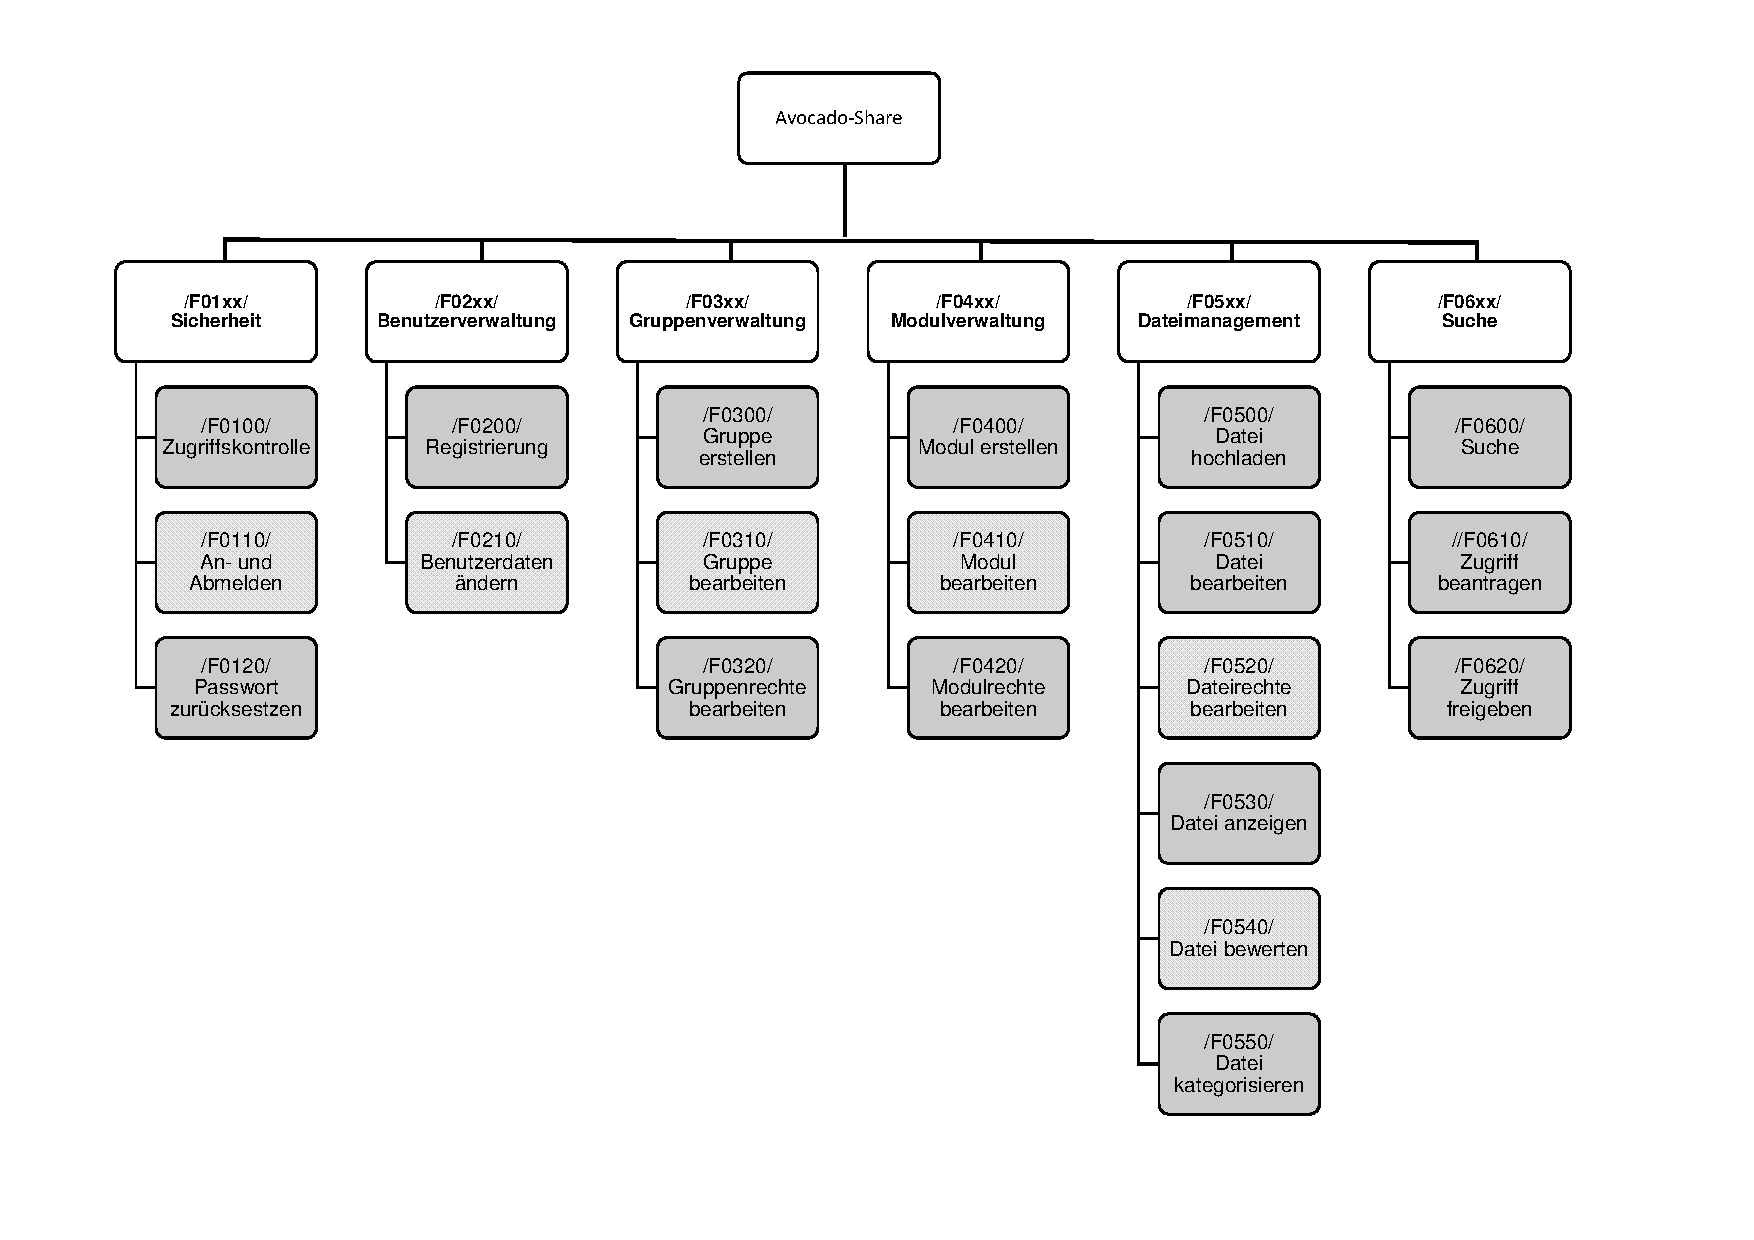
\includegraphics[width=0.8\linewidth]{Funktionsbaum.pdf}
\caption{Funktionsbaum}
\end{figure}
\end{landscape}
\requirementsection{R}{Nicht-funktionale Anforderungen}
Alle nicht-funktionalen Anforderungen \texttt{/R07xx/} sind aus dem Dokument "`Nicht-funktionale Anforderungen"' von Patrick Feisthammel \cite{patfeist15nifunanf} übernommen und gegebenenfalls ergänzt worden.

\requirement{R0700}{Gebrauchsfähigkeit (Usability)}
Die Webseiten müssen durch den Benutzer, welcher dem Benutzerprofil entspricht, ohne weitere Hilfe verwendet werden können. Es müssen, wenn der Benutzer diese für sein Verständnis benötigt, Hinweisfelder eingeblendet werden können.
Erweiterte Usability, wie zum Beispiel eine Erweiterungen für Blinde, wird nicht speziell berücksichtigt.

\requirement{R0710}{Fehlertoleranz}
Hinweise und Fehlermeldungen müssen für den Benutzer verständlich formuliert sein und eine Hilfestellung zur Problemlösung beinhalten. Kein auftretender Fehler darf dem Benutzer ohne Verarbeitung angezeigt werden.

\requirement{R0720}{Sprache und länderspezifische Einstellungen}
Die Webseiten sind in deutscher Sprache (Schweiz) verfasst und verwenden den Zeichensatz \gls{utf8}. Es werden die Schweiz-spezifischen Einstellungen von Datum, Zeit, Zahlen und Währung verwendet.

\requirement{R0730}{Zielplattform (Server)}
Die Web-Applikation muss als \gls{JSP} auf dem zur Verfügung gestellten virtuellen Server unter Verwendung einer SQL-Datenbank mit Apache Tomcat betrieben werden.

\requirement{R0740}{Zielplattform (Client)}
Die Webseiten werden in der aktuellsten freigegebenen Version des Mozilla Firefox und Google Chrome korrekt dargestellt. Die Webseite muss für Bildschirmgrössen mit einer Breite ab 480 Pixel problemlos darstellbar sein. Für Bildschirme mit einer Breite unter 600 Pixel muss eine Mobilansicht bereitstehen. Die Webseite muss skalierbar sein und sich an die Bildschrirmbreite anpassen.

\requirement{R0750}{Werkzeuge zur Entwicklung}
Als Projektmanagement-Tool und zur Verwaltung des Sourcecodes und der Dokumente muss der zur Verfügung gestellte Github-Server verwendet werden.

\requirement{R0760}{Robustheit}
Auch nach einem Neustart des virtuellen Servers muss die Webseite voll funktionsfähig sein.

\requirement{R0770}{Testbarkeit}
Für die Durchführung der Tests und der Abnahme müssen sinnvolle Testdaten in genügendem Umfang zur Verfügung gestellt werden.

\requirementsubsection{R08}{Weitere Anforderungen}
\requirement{R0800}{Sicherheit}
Die Benutzerdaten und Dateien müssen mit einem Mindestmass an Sicherheit geschützt sein. Das heisst, dass Unbefugte nur unter einem grossen Aufwand an sicherheitsrelevante Daten kommen. Benutzerpasswörter werden nicht im Klartext gespeichert, sondern sie werden mit einem Salt kombiniert und mit Hilfe eines starken, kryptographischen \gls{Hash-Algorithmus}, wie SHA-256 oder SHA-512, in einen Hash umgewandelt. Hochgeladene Dateien werden unverschlüsselt abgespeichert.

\requirement{R0810}{Verbindungssicherheit}
Um das Abhören von Passwörtern möglichst zu vermeiden, muss die HTTP-Verbindung zwischen Client und Server mit \gls{TLS} 1.2 gesichert werden. Der verwendete Algorithmus muss \gls{Perfect Forward Secrecy} unterstützen. Das Serverzertifikat muss dabei nicht von Zertifizierungsstellen verifiziert sein.

\requirement{R0820}{Antwortzeit}
Eine browserseitige Anfrage auf eine Webseite muss, falls in folgendem Text nicht anders definiert, vom Server innerhalb von maximal einer Sekunden bearbeitet und beantwortet werden. In die Antwortzeit wird weder die Übertragungszeit noch die Zeit, die der Browser benötigt, um die Webseite anzuzeigen, eingerechnet. Anfragen, eine Datei herunterzuladen (siehe \refreq{Datei anzeigen}), dürfen maximal 5 Sekunden dauern, bis der Download startet. Eine Suche muss innerhalb von maximal 5 Sekunden beantwortet werden. Aktionen, welche eine längere Rechenzeit auf dem Server beanspruchen, müssen asynchron zur Webseiten-Anfrage bearbeitet werden.


\iffalse
\begin{table}[H]
\centering
\begin{tabular}{|l|l|} \hline
\textbf{Seitenaufruf} & \textbf{Maximale Antwortzeit} & \textbf{Funktionale Anforderung}\\ \hline
Allgemein 					& 1 Sekunde  & \\ \hline
Start eines Datei-Downloads & 5 Sekunden & \refreq{Datei anzeigen}\\ \hline
Suche						& 5 Sekunden & \refreq{Suche}\\ \hline
\end{tabular}
\caption{Maximale Antwortzeit von Seitenaufrufen.}
\end{table}
\fi

\requirement{R0830}{Wiederherstellbarkeit}
Von den Systemdateien und den Dateien der Benutzer müssen von Zeit zu Zeit Sicherungskopien erstellt werden, sodass bei einem Dateiverlust im Hauptsystem ein Grossteil der verlorenen Daten wieder hergestellt werden kann. 

\requirement{R0840}{Erweiterbarkeit}
Die Systemkomponenten müssen so implementiert sein, dass diese zu einem späteren Zeitpunkt ohne grossen Mehraufwand erweitert und auf neue Bedürfnisse abgestimmt werden können. Texte müssen zentral gespeichert werden, dass sie einfach in andere Sprachen übersetzt werden könne.

\requirement{R0850}{Dokumentation in Quellcode}
Im Quellcode müssen alle Methoden, Klassen und Datenfelder dokumentiert werden.
%%%%%%%%%%%%%%%%%%%%%%%%%%%%%%%%%%%%%%%%%%%%%%%%%%%%%%%%%%%%%%%%%%%%%%%%%%%%%%%
\requirementsection{T}{Abnahmekriterien}
%%%%%%%%%%%%%%%%%%%%%%%%%%%%%%%%%%%%%%%%%%%%%%%%%%%%%%%%%%%%%%%%%%%%%%%%%%%%%%%

%%%%%%%%%%%%%%%%%%%%%%%%%%%%%%%%%%%%%%%%%%%%%%%%%%%%%%%%%%%%%%%%%%%%%%%%%%%%%%%
\requirementsubsection{T01}{Sicherheit}
%%%%%%%%%%%%%%%%%%%%%%%%%%%%%%%%%%%%%%%%%%%%%%%%%%%%%%%%%%%%%%%%%%%%%%%%%%%%%%%

%%%%%%%%%%%%%%%%%%%%%%%%%%%%%%%%%%%%%%%%%%%%%%%%%%%%%%%%%%%%%%%%%%%%%%%%%%%%%%%
\abnahmekriterium{Zugriffskontrolle}
%%%%%%%%%%%%%%%%%%%%%%%%%%%%%%%%%%%%%%%%%%%%%%%%%%%%%%%%%%%%%%%%%%%%%%%%%%%%%%%

\begin{abnahmefall}[Zugriff eines nicht angemeldeten Benutzers]
\ausgangssituation{
Ein registrierter Benutzer ist nicht angemeldet.
}
\ereignis{
Der Benutzer versucht irgend eine Seite der Applikation zu öffnen, abgesehen von der Seite zur Registrierung (/F0200/ Registrierung) und der Login Seite (\refreq{An- und Abmelden}).
}
\ergebnis{
Der Benutzer wird auf die Login Seite umgeleitet und es wird eine Fehlermeldung angezeigt, dass er angemeldet sein muss um diese Seite zu öffnen.
}
\end{abnahmefall}
%%%%%%%%%%%%%%%%%%%%%%%%%%%%%%%%%%%%%%%%%%%%%%%%%%%%%%%%%%%%%%%%%%%%%%%%%%%%%%%
\begin{abnahmefall}[Zugriff eines angemeldeten Benutzers mit Berechtigung]
	\ausgangssituation{
		Ein angemeldeter Benutzer und besitzt die erforderlichen Berechtigungen eine Seite aufzurufen. Beispielsweise besitzt er das Vewaltungsrecht einer Gruppe, dann hat er Zugriffsberechtigung auf die Seite zum Editieren der Eigenschaften dieser Gruppe.
	}
	\ereignis{
		Der Benutzer versucht irgendeine Seite der Applikation zu öffnen, auf welche er die Zugriffsberechtigung hat.
	}
	\ergebnis{
		Die vom Benutzer aufgerufene Seite wird angzeigt.
	}
\end{abnahmefall}
%%%%%%%%%%%%%%%%%%%%%%%%%%%%%%%%%%%%%%%%%%%%%%%%%%%%%%%%%%%%%%%%%%%%%%%%%%%%%%%
\begin{abnahmefall}[Zugriff eines angemeldeten Benutzers ohne Berechtigung]
	\ausgangssituation{
		Ein angemeldeter Benutzer hat keine Zugriffsberechtigung auf die Seite hat, die er öffnen will. Hat er zum Beispiel nur Leserecht an einer Gruppe, so hat er keine Zugriffsberechtigung auf die Seite zum Editieren der Eigenschaften einer Gruppe.
	}
	\ereignis{
		Der Benutzer versucht irgendeine Seite der Applikation zu öffnen, auf welche er keine Zugriffsberechtigung hat.
	}
	\ergebnis{
		Die vom Benutzer aufgerufene Seite wird nicht angezeigt und es wird eine Fehlermeldung angezeigt, dass der Benutzer die benötigten Rechte zum Aufrufen der Seite nicht besitzt.
	}
\end{abnahmefall}
%%%%%%%%%%%%%%%%%%%%%%%%%%%%%%%%%%%%%%%%%%%%%%%%%%%%%%%%%%%%%%%%%%%%%%%%%%%%%%%
\begin{abnahmefall}[Verwaltungsrecht erteilen/entziehen]
	\ausgangssituation{
		Ein angemeldeter Benutzer \user{1} besitzt Verwaltungsrecht an einem Objekt.
		Es existiert ein anderer Benutzer \user{2}, der auch Verwaltungsrecht an diesem Objekt besitzt.
		Keiner der beiden Benutzer (\user{1} oder \user{2}) ist der Ersteller des Objektes.
	}
	\ereignis{
		Der Benutzer \user{1} erteilt einem anderen Benutzer \user{3} Verwaltungsrecht am Objekt und entzieht dem Benutzer \user{2} das Verwaltungsrecht am Objekt.
	}
	\ergebnis{
		Der Benutzer \user{3} hat nun Verwaltungsrecht am erwähnten Objekt.
		Der Versuch zum Entziehen der Verwaltungsrechte des Benutzers \user{2} scheiter und es wird eine Fehlermeldung ausgegeben, da der Benutzer \user{1} nicht Ersteller des Objektes ist.
	}
\end{abnahmefall}
%%%%%%%%%%%%%%%%%%%%%%%%%%%%%%%%%%%%%%%%%%%%%%%%%%%%%%%%%%%%%%%%%%%%%%%%%%%%%%%
\begin{abnahmefall}[Verwaltungsrecht erteilen/entziehen]
	\ausgangssituation{
		Ein angemeldeter Benutzer \user{1} besitzt Verwaltungsrecht an einem Objekt.
		Es existiert ein anderer Benutzer \user{2}, der auch Verwaltungsrecht an
		diesem Objekt besitzt. Keiner der beiden Benutzer (\user{1} oder \user{2}) ist
		der Ersteller des Objektes.
	}
	\ereignis{
		Der Benutzer \user{1} erteilt einem anderen Benutzer \user{3} Verwaltungsrecht
		am Objekt und entzieht dem Benutzer \user{2} das Verwaltungsrecht am Objekt.
	}
	\ergebnis{
		Der Benutzer \user{3} hat nun Verwaltungsrecht am erwähnten Objekt. Der
		Versuch zum Entziehen der Verwaltungsrechte des Benutzers \user{2}
		scheiter und es wird eine Fehlermeldung ausgegeben, da der
		Benutzer \user{1} nicht Ersteller des Objektes ist.
	}
\end{abnahmefall}
%%%%%%%%%%%%%%%%%%%%%%%%%%%%%%%%%%%%%%%%%%%%%%%%%%%%%%%%%%%%%%%%%%%%%%%%%%%%%%%
\abnahmekriterium{An- und Abmelden}
%%%%%%%%%%%%%%%%%%%%%%%%%%%%%%%%%%%%%%%%%%%%%%%%%%%%%%%%%%%%%%%%%%%%%%%%%%%%%%%
\begin{abnahmefall}[Anmelden]
	\ausgangssituation{
		Ein registrierter Benutzer ist nicht angemeldet.
	}
	\ereignis{
		Der Benutzer öffnet die Applikation, es wird ein Anmeldeformular
		angezeigt, in welches der Benutzer seine E-Mail-Adresse und sein
		Passwort eingibt.
	}
	\ergebnis{
		Falls seine Eingaben korrekt sind, wird der Benutzer angemeldet
		und auf die Hauptseite umgeleitet. Falls die Eingaben fehlerhaft
		sind, wird eine Fehlermeldung angezeigt und der Benutzer kann es
		erneut versuchen. Zudem wird ein Link angezeigt um sein Passwort
		zurückzusetzten.
	}
\end{abnahmefall}
%%%%%%%%%%%%%%%%%%%%%%%%%%%%%%%%%%%%%%%%%%%%%%%%%%%%%%%%%%%%%%%%%%%%%%%%%%%%%%%
\begin{abnahmefall}[Anmelden]
	\ausgangssituation{
		Ein Benutzer ist registriert und angemeldet.
	}
	\ereignis{
		Der angemeldete Benutzer meldet sich über eine Schaltfläche ab.
	}
	\ergebnis{
		Der Benutzer ist abgemeldet und wird auf die Startseite der Applikation umgeleitet.
	}
\end{abnahmefall}
%%%%%%%%%%%%%%%%%%%%%%%%%%%%%%%%%%%%%%%%%%%%%%%%%%%%%%%%%%%%%%%%%%%%%%%%%%%%%%%
\abnahmekriterium{Passwort zurücksetzen}
%%%%%%%%%%%%%%%%%%%%%%%%%%%%%%%%%%%%%%%%%%%%%%%%%%%%%%%%%%%%%%%%%%%%%%%%%%%%%%%
\begin{abnahmefall}[]
	\ausgangssituation{
		Ein bestehender Benutzer, welcher aus der Applikation abgemeldet ist und
		sich anmelden will, weiss sein Passwort nicht mehr.
	}
	\ereignis{
		Der abgemeldete Benutzer gibt in das Passwort zurücksetzten Formular,
		die für seinen Benutzer zutreffende E-Mail-Adresse ein und füllt danach
		das \gls{Captcha} aus und lässt sich ein neues Passwort generieren.
	}
	\ergebnis{
		Der Benutzer ist abgemeldet und wird auf die Startseite der Applikation umgeleitet.
	}
\end{abnahmefall}
%%%%%%%%%%%%%%%%%%%%%%%%%%%%%%%%%%%%%%%%%%%%%%%%%%%%%%%%%%%%%%%%%%%%%%%%%%%%%%%
\requirementsubsection{T02}{Benutzerverwaltung}
%%%%%%%%%%%%%%%%%%%%%%%%%%%%%%%%%%%%%%%%%%%%%%%%%%%%%%%%%%%%%%%%%%%%%%%%%%%%%%%
%%%%%%%%%%%%%%%%%%%%%%%%%%%%%%%%%%%%%%%%%%%%%%%%%%%%%%%%%%%%%%%%%%%%%%%%%%%%%%%
\abnahmekriterium{Registrierung}
%%%%%%%%%%%%%%%%%%%%%%%%%%%%%%%%%%%%%%%%%%%%%%%%%%%%%%%%%%%%%%%%%%%%%%%%%%%%%%%
\begin{abnahmefall}[Registrierung]
	\ausgangssituation{
		Ein Benutzer ist noch nicht im System erfasst und will sich neu registrieren.
	}
	\ereignis{
		Der Benutzer gibt im Registrierungs-Formular seinen Vor- und Nachnamen, seine E-Mail-Adresse und sein gewünschtes Passwort ein und schliesst die Registrierung über die entsprechende Schaltfläche ab.
	}
	\ergebnis{
		Falls alle Angaben gemacht wurden und die E-Mail-Adresse ein gültiges Format hat, wird dem Benutzer eine E-Mail zur Bestätigung gesendet, mit welcher er sein Konto aktivieren kann. Falls die Angaben nicht korrekt waren, wird das Formular nochmals angezeigt und eine Fehlermeldung ausgegeben. In der Bestätigungs-E-Mail ist ein Link zum Aktivieren des Benutzerkontos enthalten und eine kurze Beschreibung über den Nutzen dieses Links.
	}
\end{abnahmefall}
%%%%%%%%%%%%%%%%%%%%%%%%%%%%%%%%%%%%%%%%%%%%%%%%%%%%%%%%%%%%%%%%%%%%%%%%%%%%%%%
\begin{abnahmefall}[Registrierung bestätigen]
	\ausgangssituation{
		Ein Benutzer hat die Registrierung abgeschlossen hat und bekam ein E-Mail, in welchem ein Link zum Aktivieren des Benutzerkontos enthalten ist.
	}
	\ereignis{
		Der Benutzer klickt im E-Mail auf den Link zur Aktivierung.
	}
	\ergebnis{
		Beim Öffnen des Links, wird man auf die Applikations-Seite weitergeleitet und der entsprechende Benutzer freigeschaltet. Dem Benutzer wird nun ein Loginformular und eine Bestätigung der Aktivierung angezeigt.
	}
\end{abnahmefall}
%%%%%%%%%%%%%%%%%%%%%%%%%%%%%%%%%%%%%%%%%%%%%%%%%%%%%%%%%%%%%%%%%%%%%%%%%%%%%%%
\abnahmekriterium{Benutzerdaten ändern}
%%%%%%%%%%%%%%%%%%%%%%%%%%%%%%%%%%%%%%%%%%%%%%%%%%%%%%%%%%%%%%%%%%%%%%%%%%%%%%%
\begin{abnahmefall}[Benutzerdaten ändern]
	\ausgangssituation{
		Ein bestehender Benutzer ist in der Applikation angemeldet.
	}
	\ereignis{
		Der Benutzer editiert über ein Formular seine Benutzerdaten, genauer gesagt seinen Vor- und Nachnamen, sein Profilbild, seine Berechtigungen und seine E-Mail-Adresse und speichert diese ab.
	}
	\ergebnis{
		 Abgesehen von der E-Mail-Adresse wurden alle Änderungen übernommen. Für die Änderung an der E-Mail-Adresse wurde an die neu eingegebene Adresse ein Bestätigungs-E-Mail gesandt, in welchem ein Link zum Bestätigen der E-Mail-Adresse enthalten ist.
	}
\end{abnahmefall}
%%%%%%%%%%%%%%%%%%%%%%%%%%%%%%%%%%%%%%%%%%%%%%%%%%%%%%%%%%%%%%%%%%%%%%%%%%%%%%%
\begin{abnahmefall}[Änderung an E-Mail bestätigen]
	\ausgangssituation{
		Ein Benutzer hat im Benutzerdaten-Änderungsformular seine E-Mail Adresse geändert und es wurde ihm an die neu eingetragene E-Mail-Adresse eine Bestätigungs-E-Mail gesandt.
	}
	\ereignis{
		Der Benutzer klickt im E-Mail auf den Link zum Validieren der geänderten E-Mail-Adresse.
	}
	\ergebnis{
		 Die E-Mail-Adresse des Benutzers wird geändert und die Startseite der Applikation wird geöffnet.
	}
\end{abnahmefall}
%%%%%%%%%%%%%%%%%%%%%%%%%%%%%%%%%%%%%%%%%%%%%%%%%%%%%%%%%%%%%%%%%%%%%%%%%%%%%%%
\begin{abnahmefall}[Benutzerkonto löschen]
	\ausgangssituation{
		Ein bestehender Benutzer ist in der Applikation angemeldet.
	}
	\ereignis{
		Der Benutzer löscht sein Benutzerkonto über eine entsprechende Schaltfläche.
	}
	\ergebnis{
		 Der Benutzer wird abgemeldet und auf die Startseite der Applikation weitergeleitet. Sein Benutzerkonto ist nun gelöscht und wenn der Benutzer versucht sich wieder anzumelden, ist dies nicht möglich.
	}
\end{abnahmefall}
%%%%%%%%%%%%%%%%%%%%%%%%%%%%%%%%%%%%%%%%%%%%%%%%%%%%%%%%%%%%%%%%%%%%%%%%%%%%%%%
\requirementsubsection{T03}{Gruppenverwaltung}
%%%%%%%%%%%%%%%%%%%%%%%%%%%%%%%%%%%%%%%%%%%%%%%%%%%%%%%%%%%%%%%%%%%%%%%%%%%%%%%
\abnahmekriterium{Gruppe erstellen}
%%%%%%%%%%%%%%%%%%%%%%%%%%%%%%%%%%%%%%%%%%%%%%%%%%%%%%%%%%%%%%%%%%%%%%%%%%%%%%%
\begin{abnahmefall}[Gruppe erstellen]
	\ausgangssituation{
		Ein bestehender Benutzer ist in der Applikation angemeldet.
	}
	\ereignis{
		Der Benutzer erstellt über ein Formular eine neue Gruppe und  konfiguriert diese sogleich (siehe \refreq{Gruppe bearbeiten}). Er bestimmt lediglich den Namen der Gruppe und schliesst das Erstellen der Gruppe ab.
	}
	\ergebnis{
		Falls keine andere Gruppe mit dem gleichen Namen bereits existiert, wird die Gruppe mit den eingegebenen Konfigurationen erstellt. Zusätzlich wird der Benutzer, welcher die Gruppe erstellt hat, gleich als Ersteller der Gruppe eingetragen, das Erstelldatum der Gruppe wird gesetzt und der Ersteller bekommt sogleich Verwaltungs-Rechte an der Gruppe. Ist der Gruppenname bereits vergeben wird dem Benutzer eine Fehlermeldung, dass bereits eine Gruppe mit dem gleichen Namen existiert, angezeigt und das Erstellformular für die Gruppe wird erneut angezeigt.
	}
\end{abnahmefall}
%%%%%%%%%%%%%%%%%%%%%%%%%%%%%%%%%%%%%%%%%%%%%%%%%%%%%%%%%%%%%%%%%%%%%%%%%%%%%%%
\abnahmekriterium{Gruppe bearbeiten}
%%%%%%%%%%%%%%%%%%%%%%%%%%%%%%%%%%%%%%%%%%%%%%%%%%%%%%%%%%%%%%%%%%%%%%%%%%%%%%%
\begin{abnahmefall}[Gruppe bearbeiten]
	\ausgangssituation{
		Es gibt eine Gruppe mit mehreren Mitgliedern. Ein angemeldeter Benutzer besitzt Verwaltungsrecht an dieser Gruppe.
	}
	\ereignis{
		Der Benutzer ändert über das Bearbeitungs-Formular der Gruppe den Namen, die Beschreibung und die Mitglieder und speichert diese Änderungen ab.
	}
	\ergebnis{
		Falls der geänderte Name nicht gleich wie der einer anderen Gruppe lautet, werden alle Änderungen an der Gruppe übernommen und die Seite mit den Eigenschaften der Gruppe angezeigt. Ansonsten wird eine Fehlermeldung ausgegeben und das Bearbeitungs-Formular wird wieder angezeigt.
	}
\end{abnahmefall}
%%%%%%%%%%%%%%%%%%%%%%%%%%%%%%%%%%%%%%%%%%%%%%%%%%%%%%%%%%%%%%%%%%%%%%%%%%%%%%%
\begin{abnahmefall}[Gruppe löschen]
	\ausgangssituation{
		Es gibt eine Gruppe mit mehreren Mitgliedern. Ein angemeldeter Benutzer besitzt Verwaltungsrecht an dieser Gruppe.
	}
	\ereignis{
		Der Benutzer ändert über das Bearbeitungs-Formular der Gruppe den Namen, die Beschreibung und die Mitglieder und speichert diese Änderungen ab.
	}
	\ergebnis{
		Falls der geänderte Name nicht gleich wie der einer anderen Gruppe lautet, werden alle Änderungen an der Gruppe übernommen und die Seite mit den Eigenschaften der Gruppe angezeigt. Ansonsten wird eine Fehlermeldung ausgegeben und das Bearbeitungs-Formular wird wieder angezeigt.
	}
\end{abnahmefall}
%%%%%%%%%%%%%%%%%%%%%%%%%%%%%%%%%%%%%%%%%%%%%%%%%%%%%%%%%%%%%%%%%%%%%%%%%%%%%%%
\abnahmekriterium{Gruppenrechte bearbeiten}
%%%%%%%%%%%%%%%%%%%%%%%%%%%%%%%%%%%%%%%%%%%%%%%%%%%%%%%%%%%%%%%%%%%%%%%%%%%%%%%
\begin{abnahmefall}[Gruppen-Berechtigungen erteilen]
	\ausgangssituation{
		Es existiert die Gruppen \group{1}, \group{2} und \group{3}, ein angemeldeter Benutzer \user{1} und die Benutzer \user{2} und \user{3}. Des weiteren gibt es Objekte an denen die Gruppe \group{1} Leserecht, Schreibrecht oder Verwaltungsrecht besitzt. Die Tabelle~\ref{tab:ausgangssituation_grippenrechte_erteilen} zeigt die Rechte der Gruppen und Benutzer an der Gruppe \group{1}.
		\\[1em]
		&
		\begin{tabular}{|l|l|} \hline
			\textbf{Inhaber des Rechts} & \textbf{Rechte an der Gruppe \group{1}} \\ \hline
			Benutzer \user{1} 			& Verwaltungsrecht \\ \hline
			Gruppe \group{2}, Benutzer \user{2} 	& Keine Rechte \\ \hline
			Gruppe \group{3}, Benutzer \user{3}  & Leserecht \\ \hline 
		\end{tabular}
		\captionof{table}{Rechte der Benutzer und Gruppen in der Gruppe \group{1}}
		\label{tab:ausgangssituation_grippenrechte_erteilen}
	}%
	\ereignis{
		Der Benutzer \user{1} erteilt dem Benutzer \user{2} und der Gruppe \group{2} Leserechte an der Gruppe \group{1}. Dem Benutzer \user{3} und der Gruppe \group{3} erteilt der Benutzer \user{1} Verwaltungsrecht an der Gruppe \group{1}.
	}%
	\ergebnis{
		Der Benutzer \user{2} und die Gruppe \group{2} übernehmen alle Berechtigungen welche die Gruppe (\group{1}) in anderen Modulen, Gruppen und Dateien besitzt. Die Gruppe \group{3} und der Benutzer \user{3} haben nun die Verwaltungsrecht an der Gruppe \group{1} und können nun deren Eigenschaften ändern (siehe Gruppe bearbeiten). 
	}
\end{abnahmefall}
%%%%%%%%%%%%%%%%%%%%%%%%%%%%%%%%%%%%%%%%%%%%%%%%%%%%%%%%%%%%%%%%%%%%%%%%%%%%%%%
\begin{abnahmefall}[Gruppen-Berechtigungen entziehen]
	\ausgangssituation{
		Es existieren die Gruppen \group{1}, \group{2} und \group{3}, ein angemeldeter Benutzer \user{1}, welcher nicht der Ersteller der Gruppe \group{1} ist, und die Benutzer \user{2} und \user{3}. Die nachfolgende Tabelle~\ref{tab:ausgangssituation_grippenrechte_entziehen} zeigt die Berechtigungen der Benutzer und Gruppen an der Gruppe \group{1}.\\[1em]
		&
		\begin{tabular}{|l|l|} \hline
		\textbf{Inhaber des Rechts} & \textbf{Rechte an der Gruppe \group{1}}\\ \hline
		Benutzer \user{1} 			& Verwaltungsrecht \\ \hline
		Gruppe \group{2}, Benutzer \user{2} 	& Leserecht \\ \hline
		Gruppe \group{3}, Benutzer \user{3}  & Verwaltungsrecht \\ \hline 
		\end{tabular}
		\captionof{table}{Rechte der Benutzer und Gruppen in der Gruppe \group{1}}
		\label{tab:ausgangssituation_grippenrechte_entziehen}
	}%
	\ereignis{
		Der Benutzer \user{1} entzieht den Gruppen \group{2} und \group{2} und den Benutzern \user{2} und \user{3} alle Rechte an der Gruppe \group{1}.
	}%
	\ergebnis{
		Der Gruppe \group{2} und dem Benutzer \user{2} werden alle Berechtigungen an der Gruppe \group{1} entzogen und somit auch alle Berechtigungen an anderen Modulen, Gruppe und Dateien, welche mit der Mitgliedschaft an der Gruppe \group{1} einhergegangen sind. Der Gruppen \group{3} und Benutzer \user{3} wird das Verwaltungsrecht an der Gruppe \group{1} nicht entzogen und dem Benutzer \user{1} wird eine Fehlermeldung ausgegeben, da der Benutzer \user{1} diese Berechtigung nicht entziehen kann.
	}%
\end{abnahmefall}
%%%%%%%%%%%%%%%%%%%%%%%%%%%%%%%%%%%%%%%%%%%%%%%%%%%%%%%%%%%%%%%%%%%%%%%%%%%%%%%

\clearpage

\glsaddall
\printglossaries

%\bibliographystyle{ieeetr}
\nocite{*}
%\bibliography{sources}
\printbibliography[heading=bibintoc]

\end{document}